\documentclass[1000pt]{article}
\pagenumbering{arabic}
\usepackage{mathptmx,amsmath}
\usepackage{pdfslide2}%,pause}
\usepackage{graphicx}
\usepackage{epstopdf}
\usepackage[T1]{fontenc} %need for portuguese caracters
\graphicspath{{./figures/}}
\usepackage{float}
\usepackage{tabularx}
\usepackage{braket}
\usepackage{multicol}
\usepackage{xcolor,colortbl}

\definecolor{itblue}{rgb}{0.0,0.0,0.5}
\definecolor{itred}{rgb}{0.82,0.18,0.24}

\definecolor{tab}{RGB}{0,82,136}
\definecolor{tab2}{RGB}{173,193,222}


\definecolor{title}{RGB}{68,85,95}
\definecolor{author}{RGB}{120,144,159}
\definecolor{author2}{RGB}{180,204,219}


\newcommand{\half}{\textstyle \frac{1}{2}}%
\newcommand{\fig}[2]{\colorbox{white}{\includegraphics[scale=#2]{#1}}}%
%\newcommand{\fig}[2]{\includegraphics[scale=#2]{#1}}%
\newcommand{\pd}[2]{\frac{\partial #1}{\partial #2}}%
\newcommand{\cb}[1]{{\color{itblue} #1}}%
\renewcommand{\labelitemi}{\textcolor{itred}{\normalsize $\bullet$}}
\renewcommand{\labelitemii}{\textcolor{green}{$\star$}}
\newcommand{\ave}[1]{\langle #1 \rangle}%
\newcommand{\mysection}[1]{\section*{\color{black}\sffamily #1}}%

\newcommand{\cref}[1]{{\fontsize{17pt}{0cm}\selectfont\color{black} #1}}%
\renewcommand*\footnoterule{}
\newcommand\blfootnote[1]{%
  \begingroup
  \renewcommand\thefootnote{}\footnote{#1}%
  \addtocounter{footnote}{-1}%
  \endgroup
}

\pagestyle{title}

\begin{document}

%------------TITLE SLIDE -------
\begin{titlepage}  \overlay{it_0.png}

\color{itblue} \sffamily \noindent \normalsize
\hspace*{4cm} Quantum Technologies, 2018/19\\
\hspace*{4cm} Physics Department, University of Aveiro\\
\\
\\
\hspace*{6.5cm}\begin{minipage}{15in}
\vspace*{2cm}
\begin{flushleft}
 \color{title} \sffamily \noindent \Huge
\textbf{Coherent One Way (COW) QKD Protocol}
\end{flushleft}
\end{minipage}
\vspace*{2cm}\\
\\
\hspace*{6.5cm}
%\begin{minipage}{7.5cm}
\color{author}
\Large João António$^1$, Daniel Pereira$^{2,3}$, Armando N. Pinto$^{2,3}$\\
%\end{minipage}\
\\
\vspace*{2cm}\\
\hspace*{6.5cm}
\begin{minipage}{12cm}
\color{title}
\large Physics Department$^1$,\\
Department of Electronics, Telecommunications and Informatics$^2$,\\
University of Aveiro, Aveiro, Portugal\\
Instituto de Telecomunica\c{c}\~{o}es,$^3$, Aveiro, Portugal
\end{minipage}\


\end{titlepage}


\mysection{\Huge\textbf{ Quantum Key Distribution}} \Large \vspace*{1cm}
\overlay{it_1.png}
\begin{itemize}
\item Quantum Key Distribution (QKD) is a secure way of create and share a unique random key between two spatially distant parties. 
\item Polarization QKD vs Time Bin QKD.
\end{itemize}
They use:
\begin{itemize}
\item One quantum channel (with one way transmission)
\item And one authenticated classic channel (can be eavesdropped but can't be modified).
\end{itemize}
  \begin{figure}[hbt]
    	\centering
    	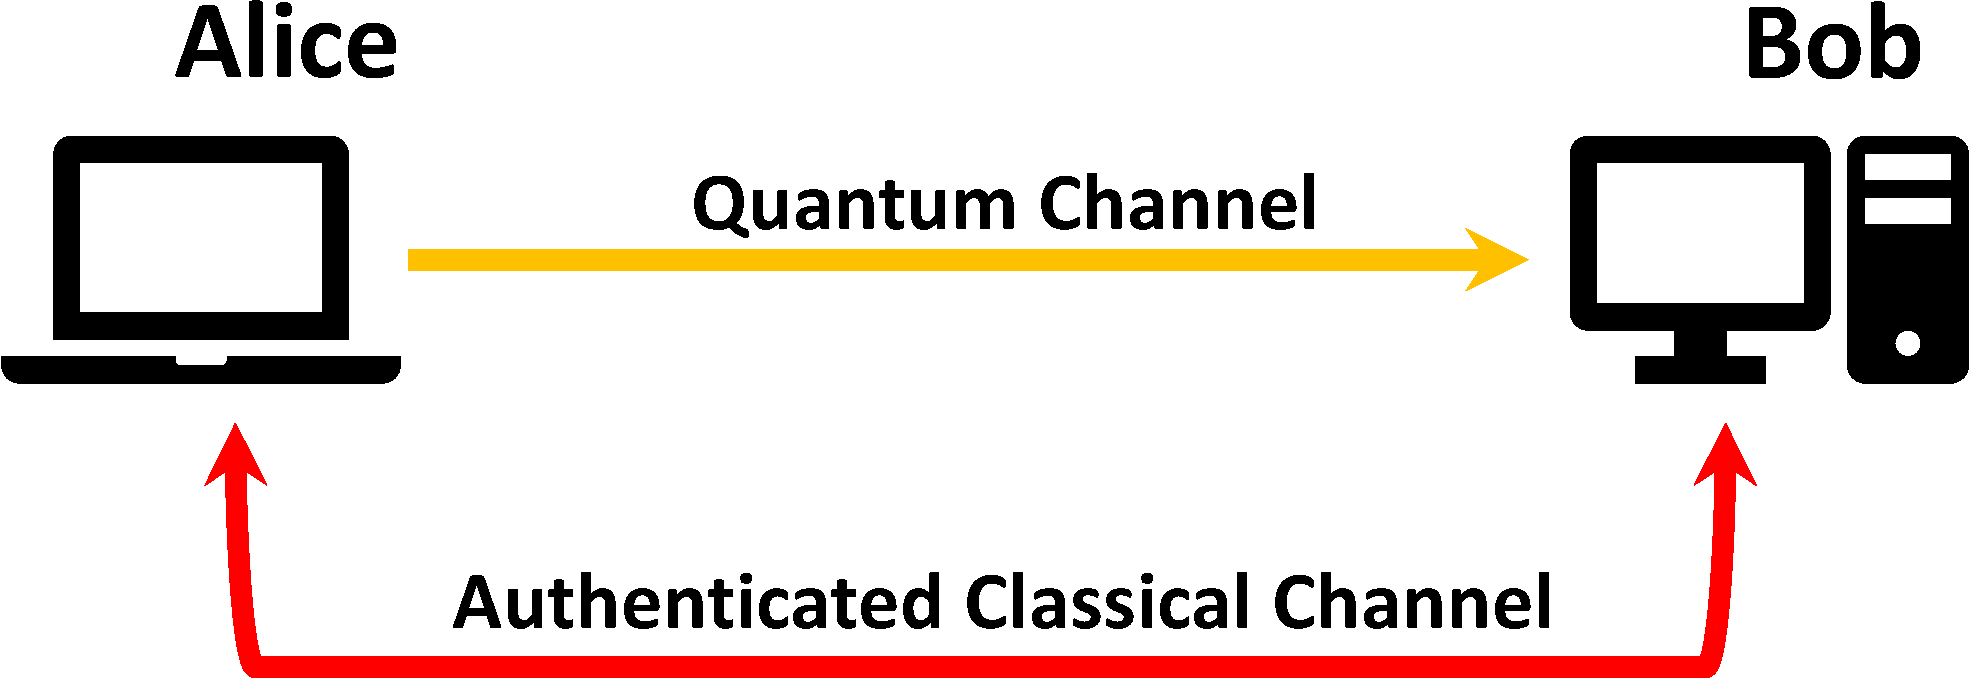
\includegraphics[width=0.3\textwidth]{./figures/Full.pdf}
    \end{figure}
    
    
\blfootnote{
\hspace*{12cm}
\begin{minipage}{26cm}
\cref{
Ouellette, Jennifer. "Quantum key distribution." Industrial Physicist 10.6 (2004): 22-25.
}
\end{minipage}

}
%%%%%%%%%%%%%%%%%%%%%%%%%%%%%%
%------------ SLIDE 1 -------%
%%%%%%%%%%%%%%%%%%%%%%%%%%%%%%
\mysection{\Huge\textbf{Time Bin QKD}} \Large \vspace*{1cm}
\begin{itemize}

\item The Coherent One Way (COW) protocol was elaborated by Nicolas Gisin et al in 2004. 

\item Uses time bin encoding.

\item It is has a very simple setup.
\end{itemize}
    \begin{figure}[hbt]
    	\centering
    	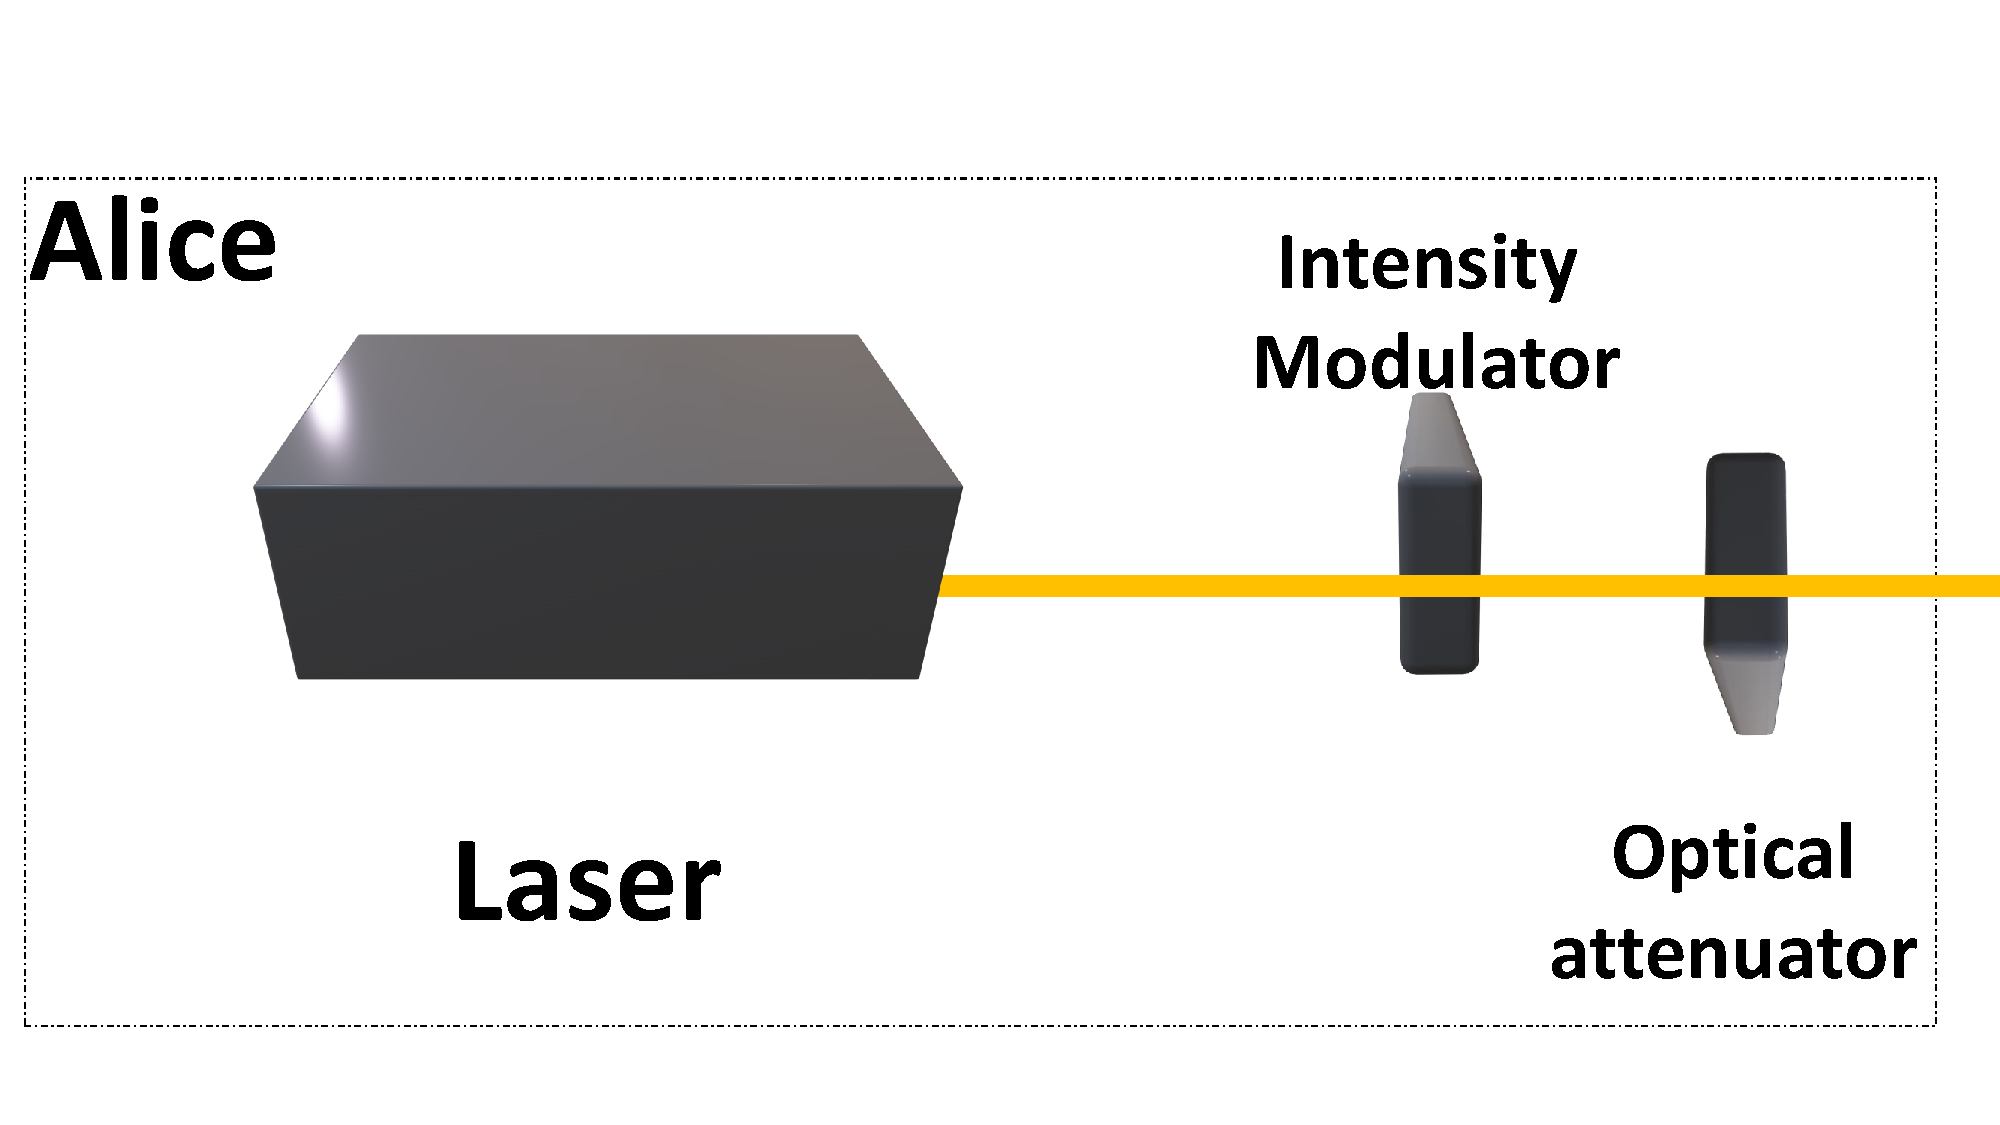
\includegraphics[width=0.4\textwidth]{./figures/A.pdf}
        	\label{bob}
    \end{figure}
    
\blfootnote{
\hspace*{12cm}
\begin{minipage}{26cm}
\cref{
Gisin, Nicolas, et al. "Towards practical and fast quantum cryptography." arXiv preprint quant-ph/0411022 (2004)
}
\end{minipage}
}

%%%%%%%%%%%%%%%%%%%%%%%%%%%%%%
%------------ SLIDE x -------%
%%%%%%%%%%%%%%%%%%%%%%%%%%%%%%
\mysection{\Huge\textbf{Alice - COW protocol}} \Large \vspace*{1cm}

\begin{multicols}{2}

\begin{description}
  \item[Step 1] Alice creates a random key using:  
\end{description}

$$|0\rangle = |\alpha\rangle |\emptyset\rangle =\ \ Logical\ 0\ $$
  $$|1\rangle = |\emptyset\rangle |\alpha\rangle =\ \ Logical\ 1\ $$
$$|d\rangle = |\alpha\rangle |\alpha\rangle = Decoy State$$

Where $|\emptyset\rangle$ is the vacuum state and $|\alpha\rangle$ is a coherent state of light with intensity $\mu=|\alpha|^2<<1$.

\vspace*{5cm}

\columnbreak
\hspace{-5cm}	
\vspace*{-2cm}
    	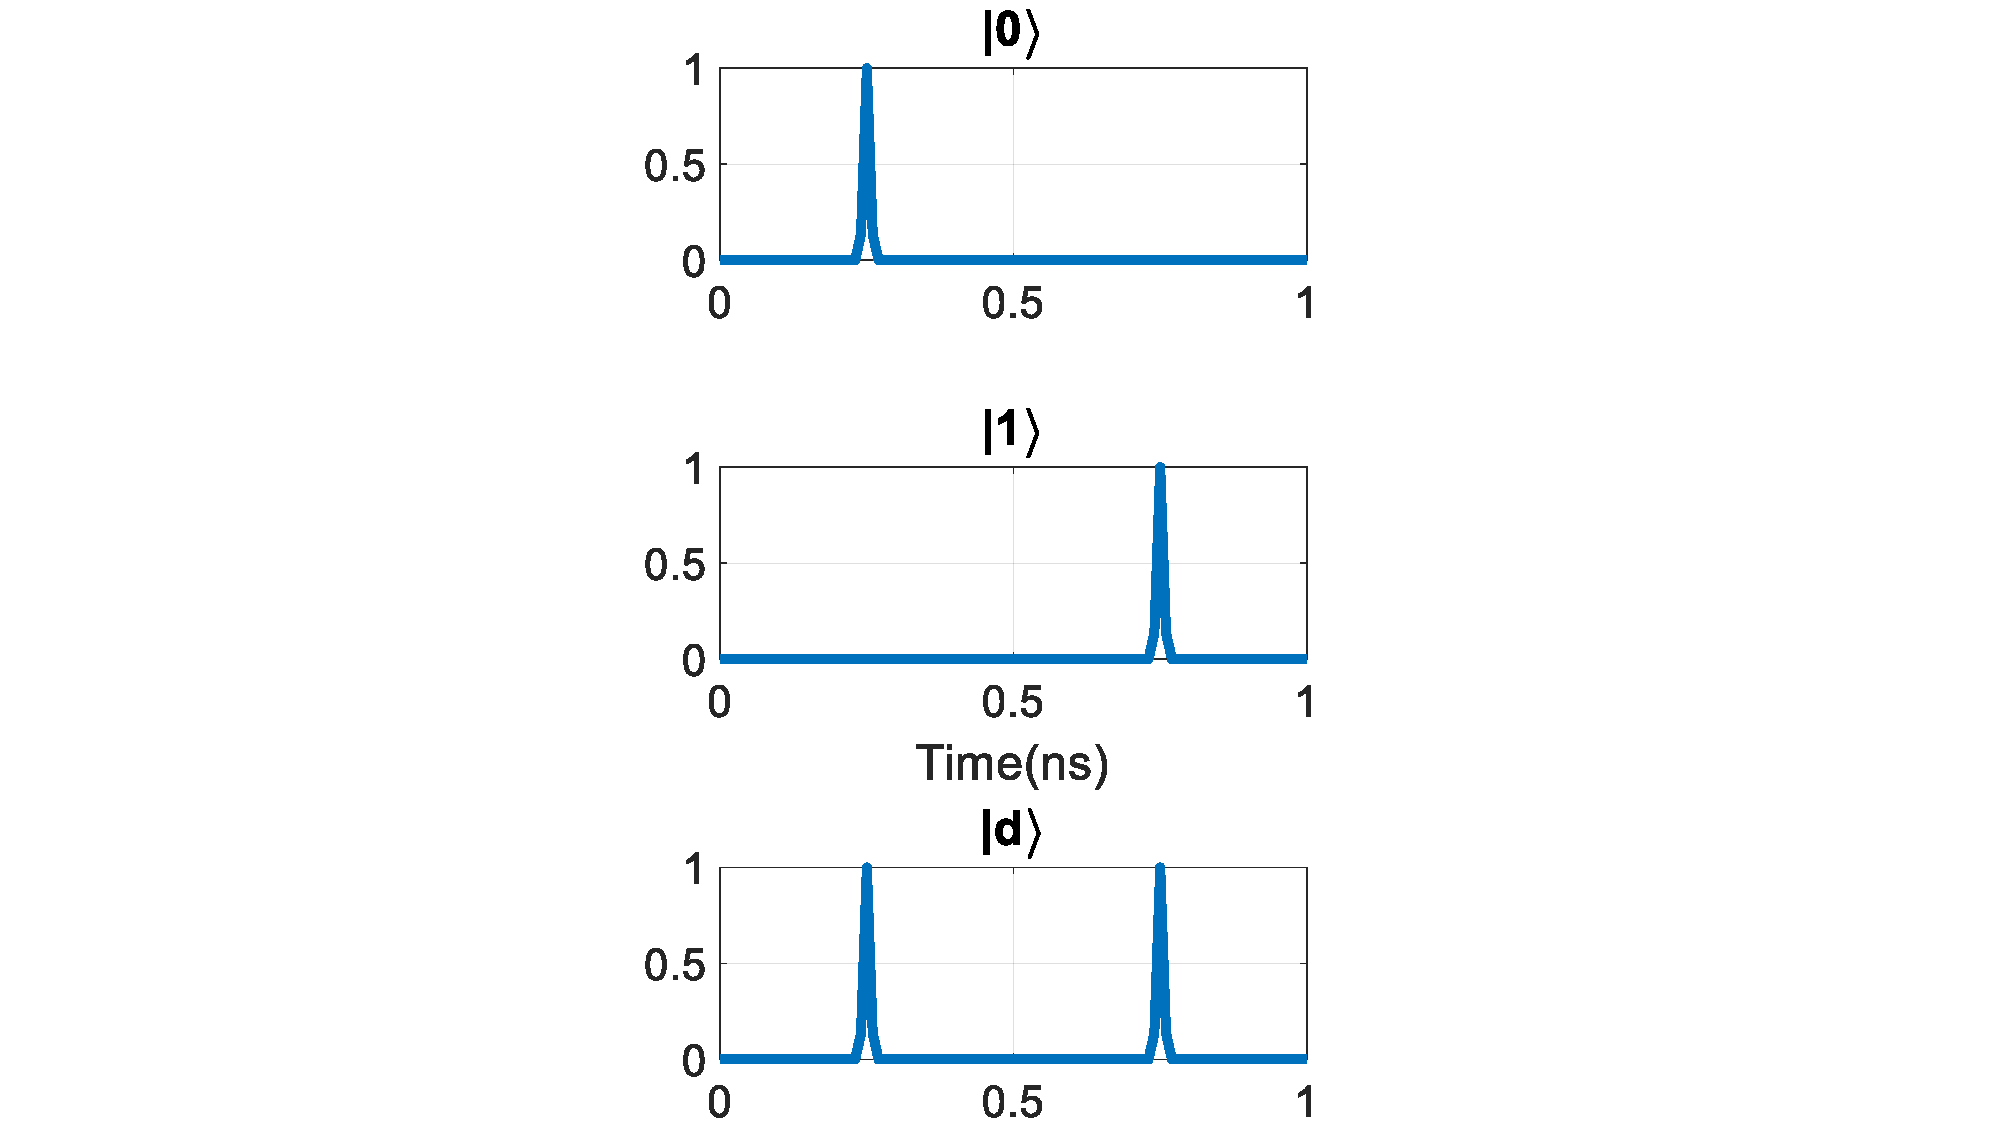
\includegraphics[width=0.7\textwidth]{./figures/S1A.pdf}
\vspace*{1cm}
\end{multicols} 

%--------------------------------------------------------------------------------------------------
%------------ SLIDE -------------------------------------------------------------------------------

\mysection{\Huge\textbf{Bob - COW protocol}} \Large \vspace*{1cm}

\begin{description}
  \item[Step 2] A fraction $t_B$ of the photons go into the photon counter $D_B$, where the bits are discriminated by the time of arrival.



\begin{multicols}{2}
Half of the other photons are delayed by 0.5 $t_{bit}$ interacting with the half of non-delayed bits.
    	\centering
    	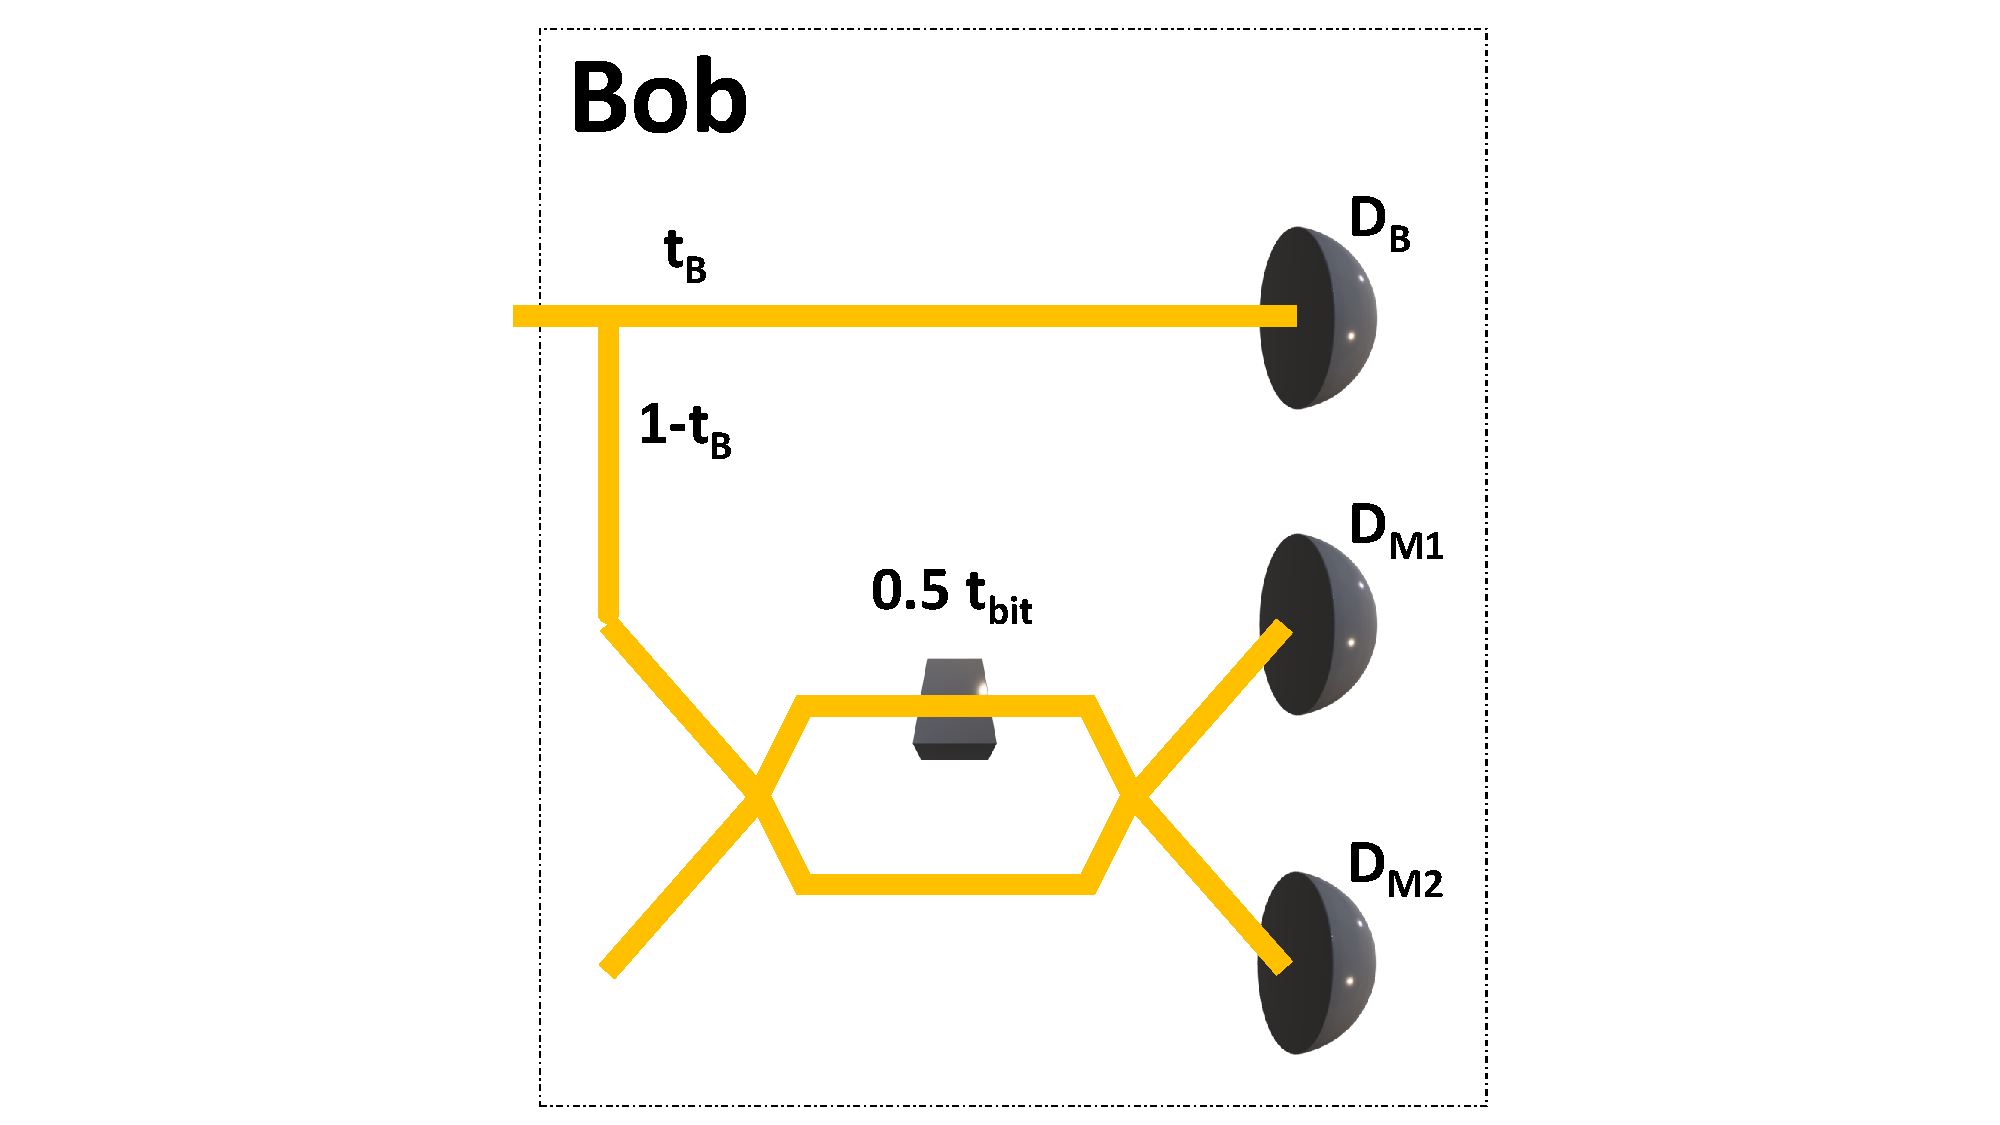
\includegraphics[width=0.5\textwidth]{./figures/B.pdf}


\columnbreak
Therefore $D_{M2}$ (constructive photon counter) should only click when:
    	\centering
    	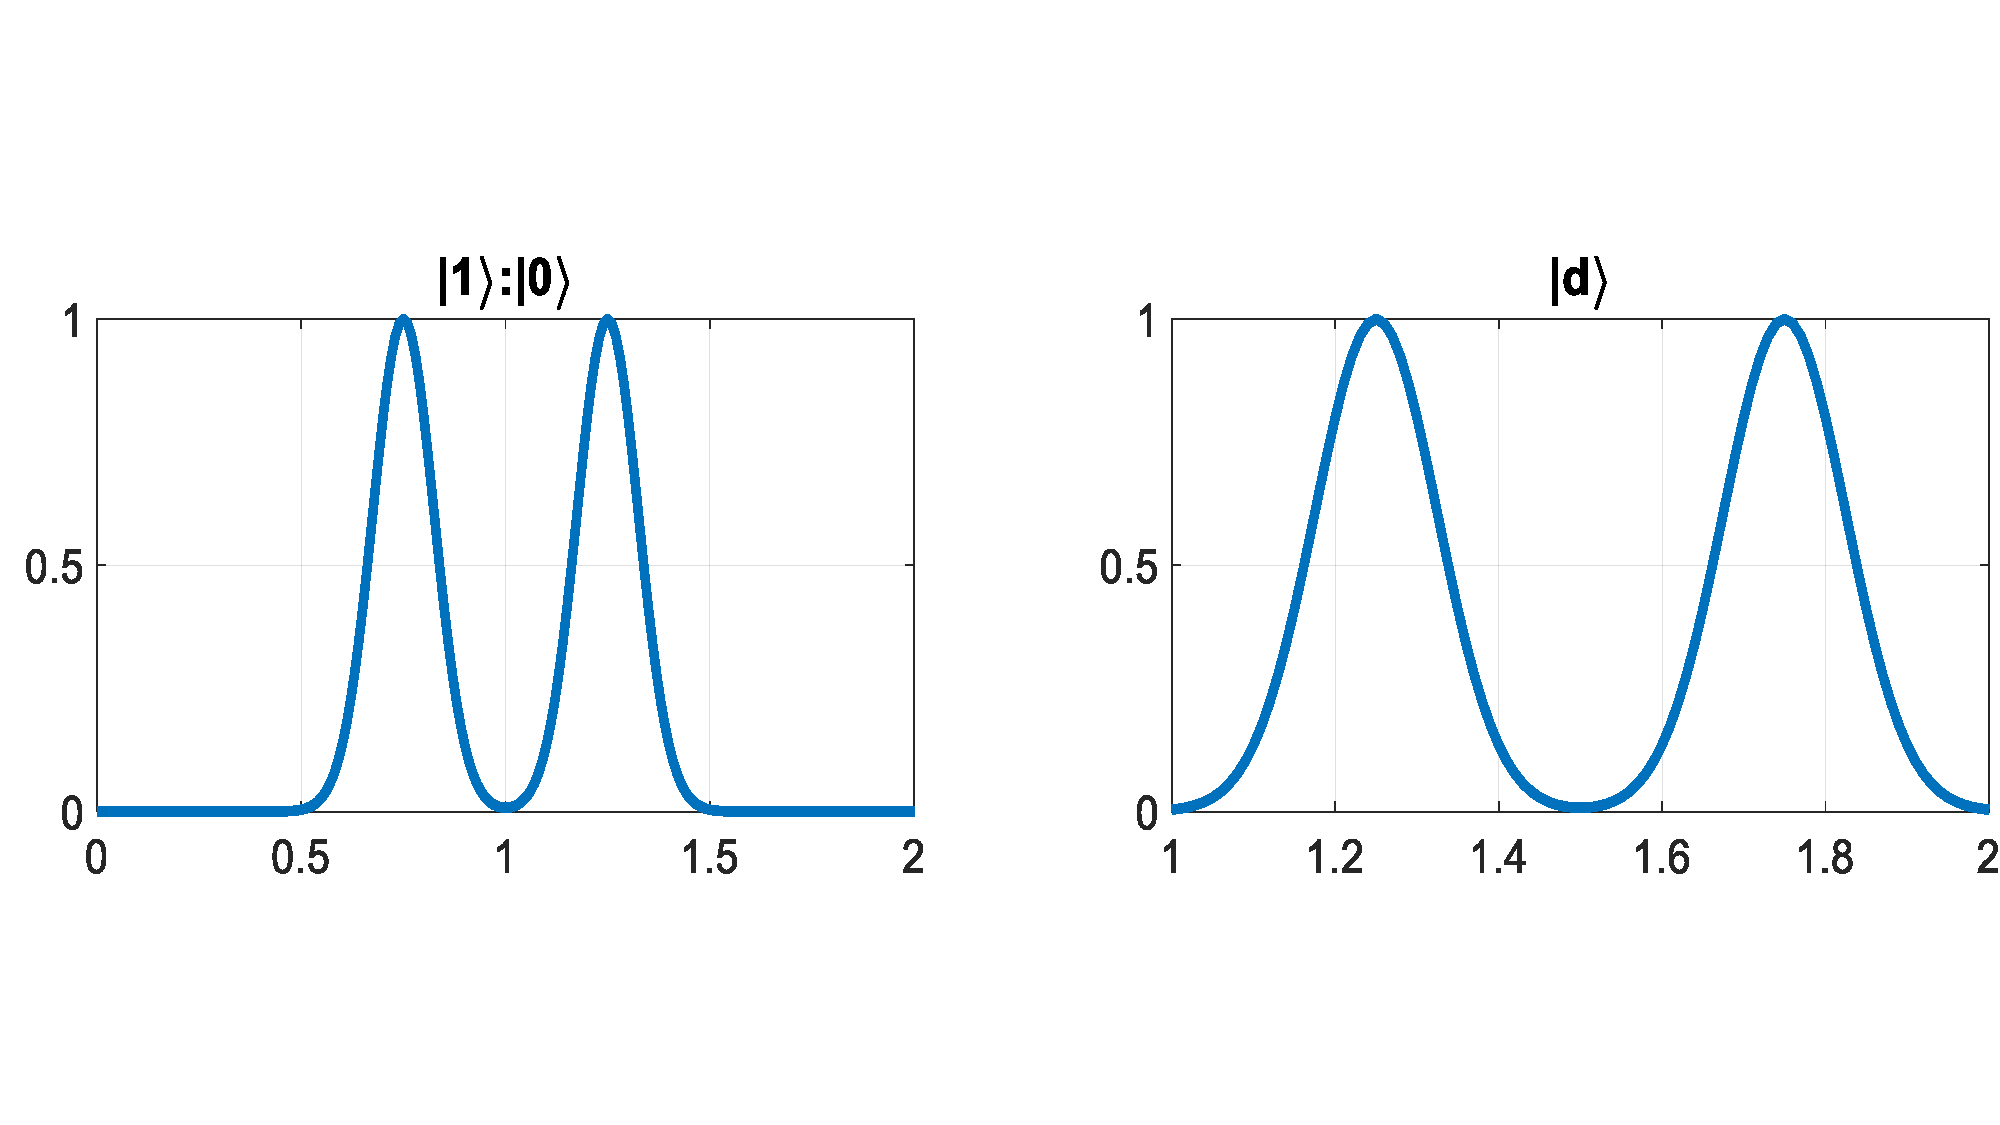
\includegraphics[width=0.5\textwidth]{./figures/S2.pdf}
    
\end{multicols}    


\end{description}  

%--------------------------------------------------------------------------------------------------
%------------ SLIDE -------------------------------------------------------------------------------

\mysection{\Huge\textbf{Monitoring line - COW protocol}} \Large \vspace*{1cm}


  \begin{figure}[hbt]
    	\centering
    	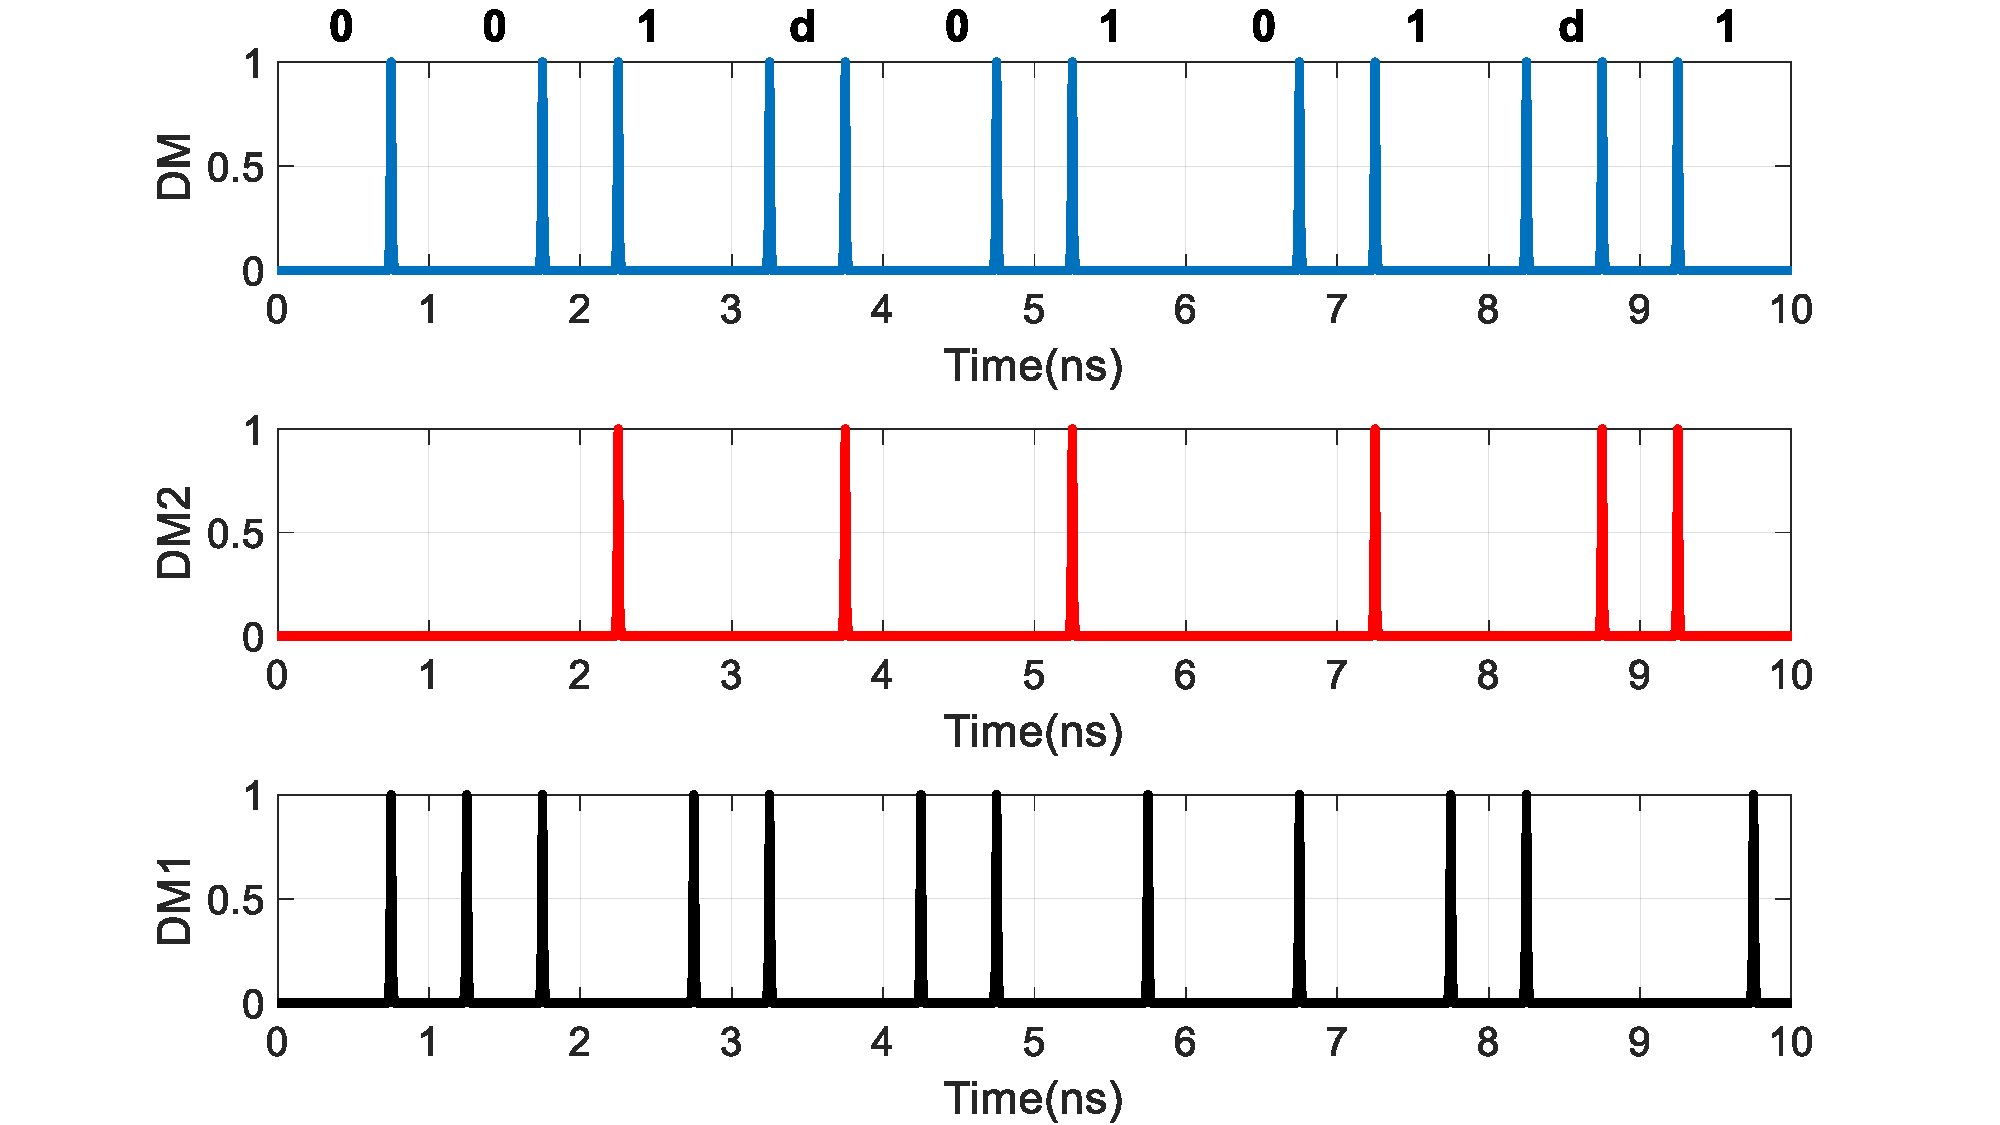
\includegraphics[width=0.75\textwidth]{./figures/DM3.pdf}
    \end{figure}

%--------------------------------------------------------------------------------------------------
%------------ SLIDE -------------------------------------------------------------------------------

\mysection{\Huge\textbf{Testing Visibility and Errors - COW protocol}} \Large \vspace*{1cm}
\begin{description}

\item [Step 3] Alice tell the decoy times. Bob checks if the $D_{M2}$ has fired during those times.

\item [Step 4] Bob reveals the other times that he had a detection in $D_{M2}$, Alice verifies if they belong to a $|1\rangle:|0\rangle$.

\item [Step 5] Bob reveals the times that $D_B$ fired, and they use those as key.

\item [Step 6] QBER, check the number of the detections for every detector.

\item [Step 7] run error correction and privacy amplification.

\begin{figure}[hbt]
    	\centering
    	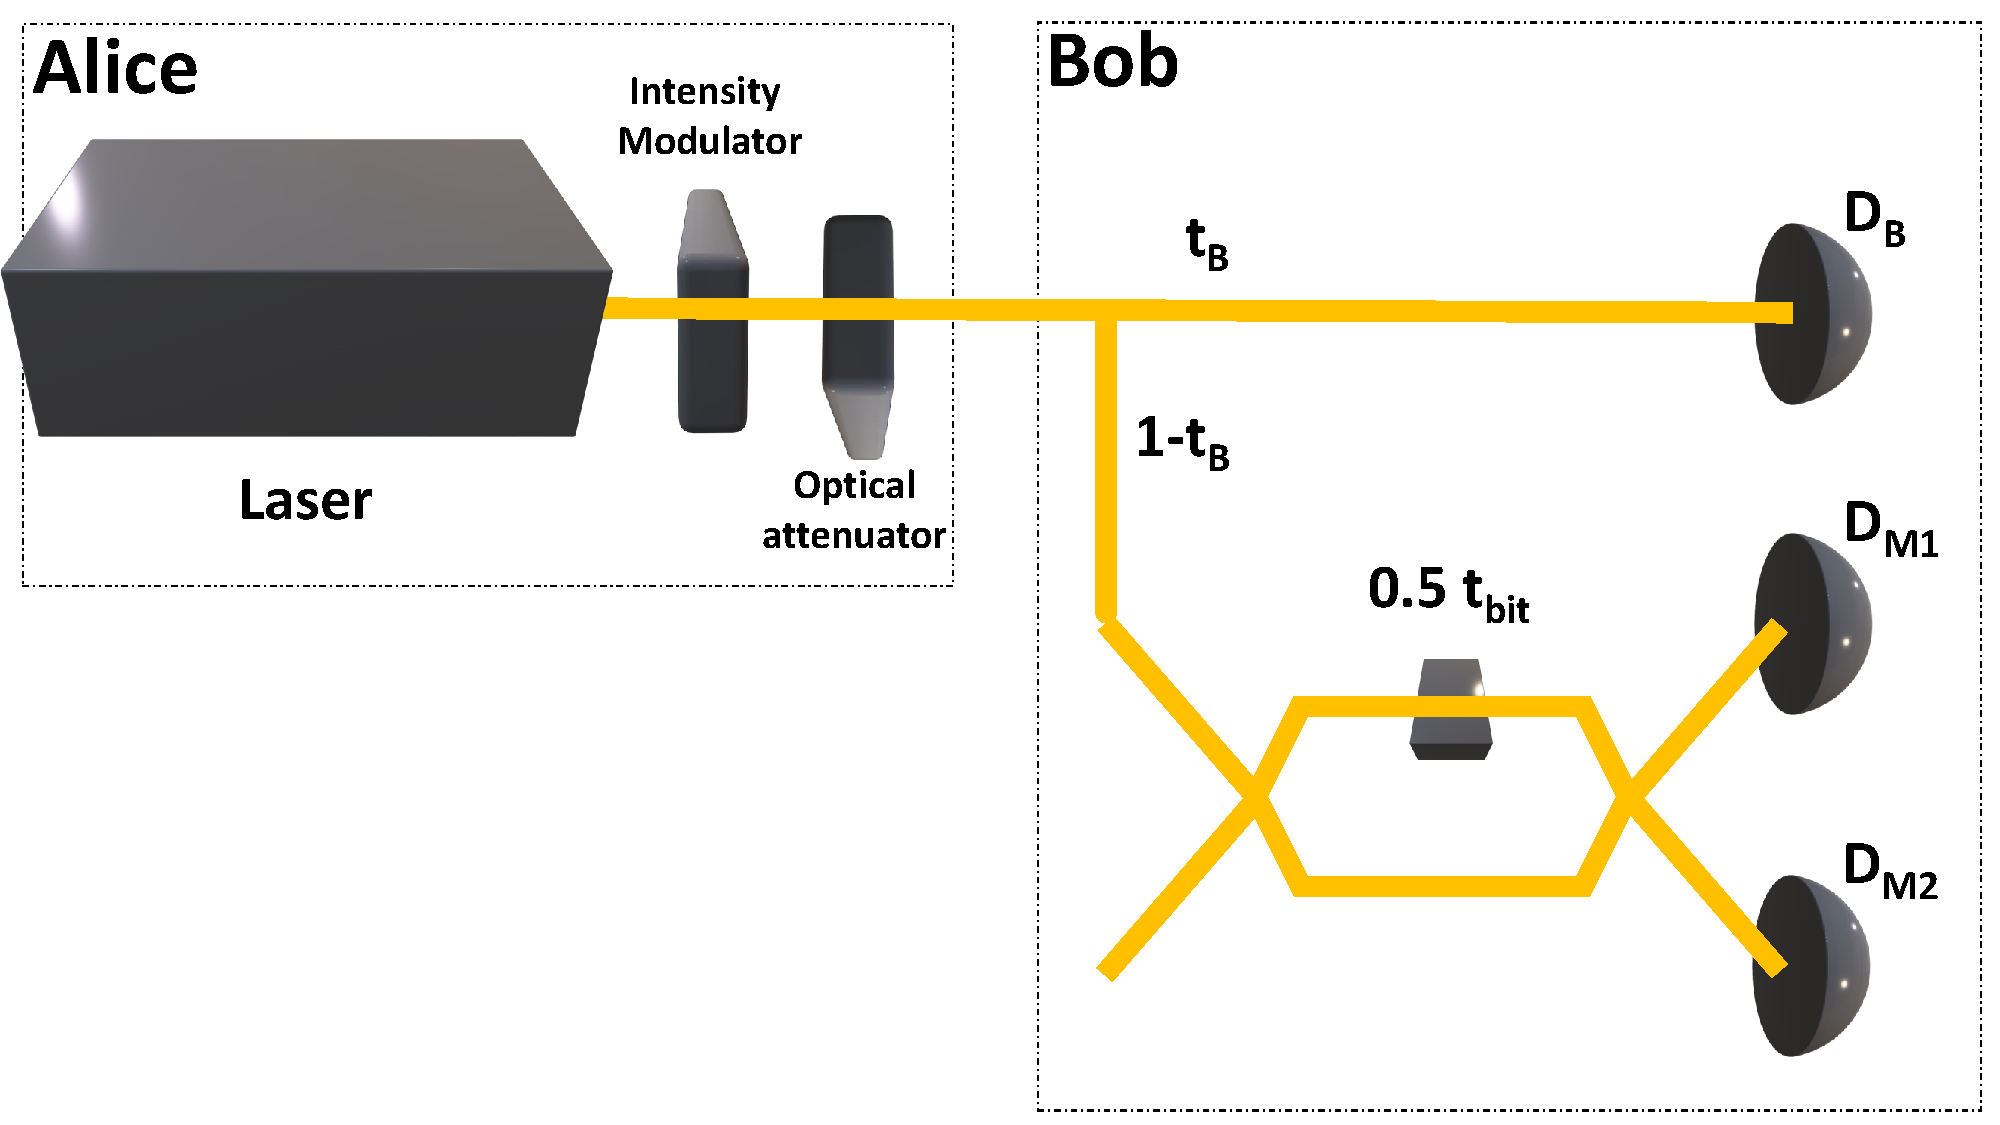
\includegraphics[width=0.4\textwidth]{./figures/Full2.pdf}
    \end{figure}
\end{description}
%--------------------------------------------------------------------------------------------------
%------------ SLIDE -------------------------------------------------------------------------------
\mysection{\Huge\textbf{Security}} \Large \vspace*{1cm}
\begin{description}
\item The two main security features of the model is the test of \textbf{coherence} and the \textbf{Length of the Key}.

\item We want to see how robust is the protocol to a \textbf{Intercept-Resend Attack}. On this attack Eve captures all the information, measures and then resend it to Bob.
\end{description}
\begin{multicols}{2}
Using the same representation as previously:

    	\centering
    	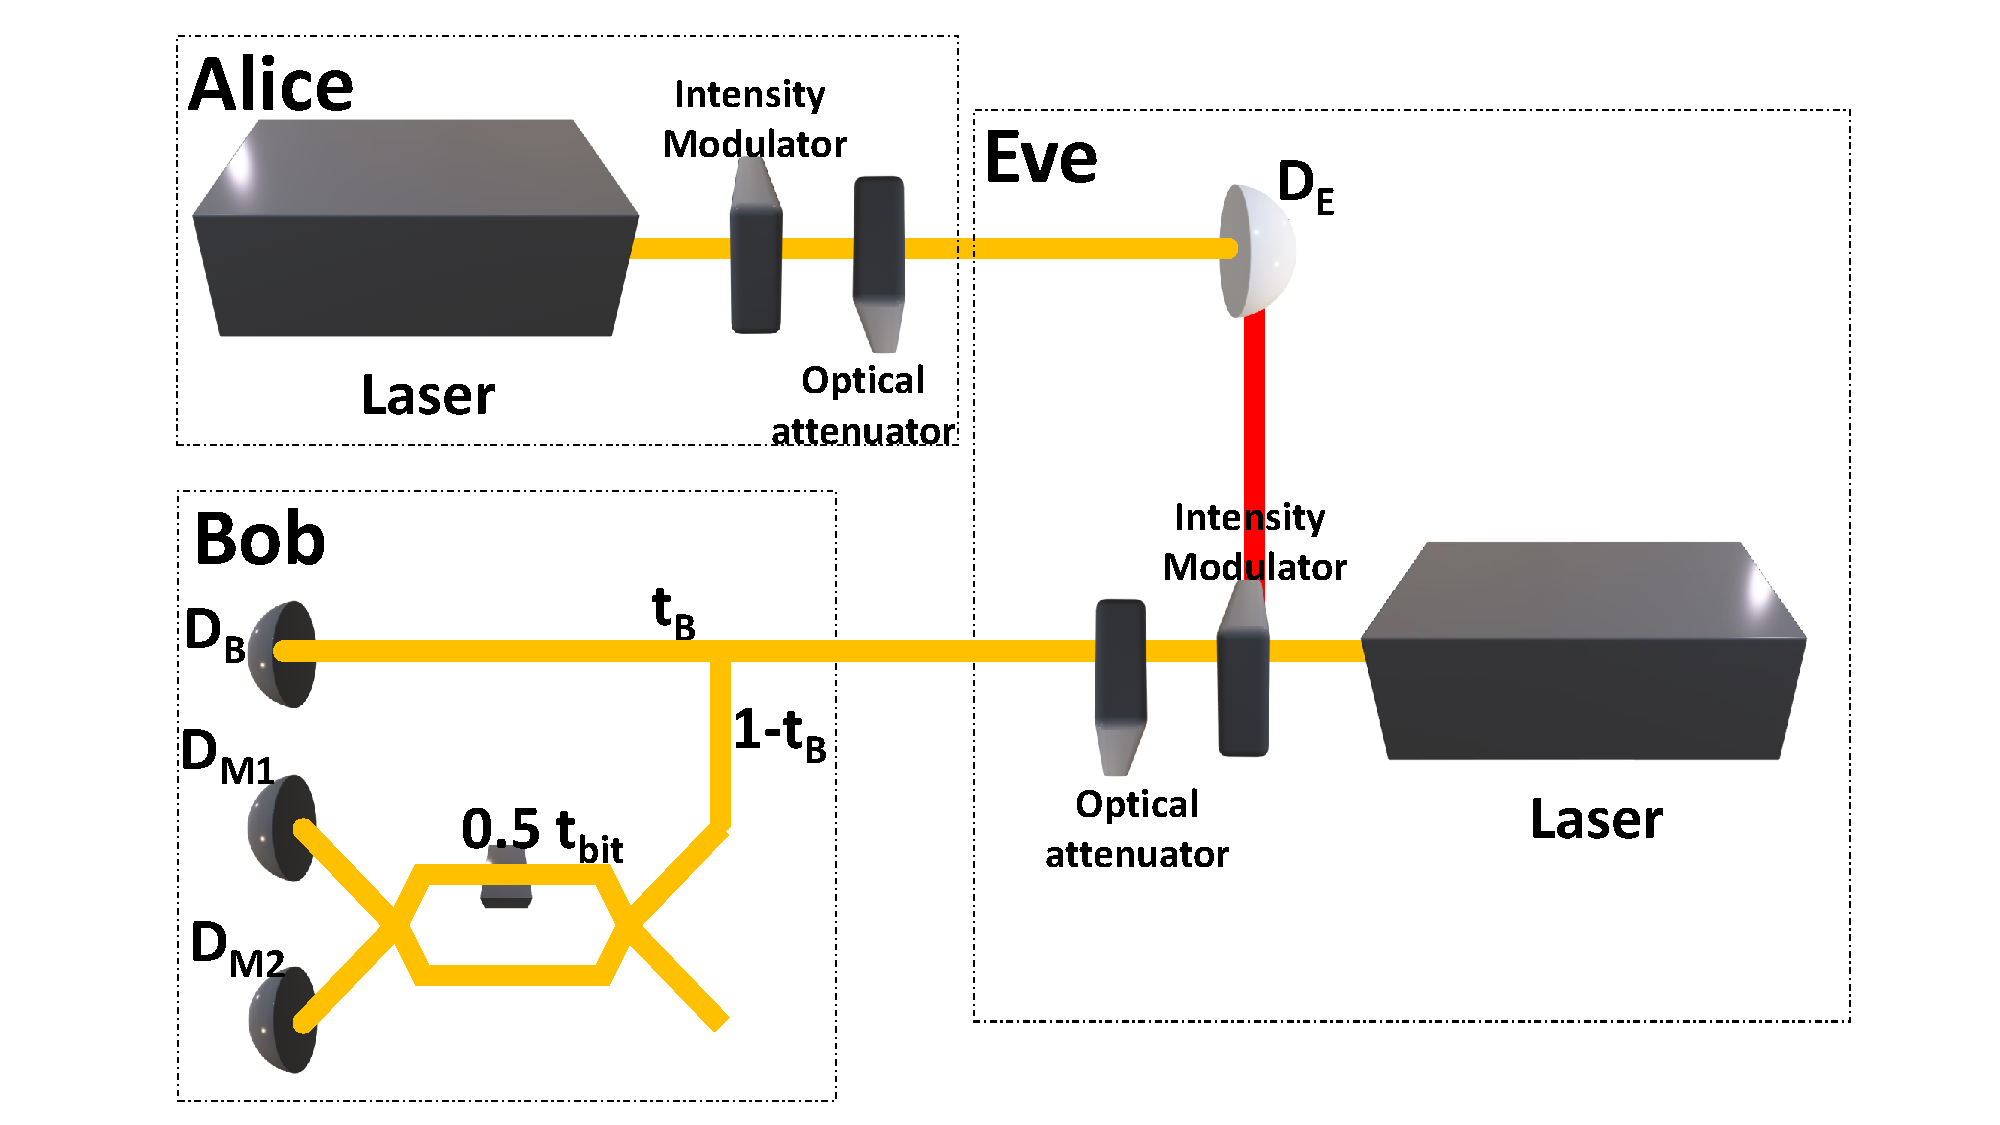
\includegraphics[width=0.5\textwidth]{./figures/E.pdf}
    \columnbreak
    
Using a block Diagram:
    	\centering
    	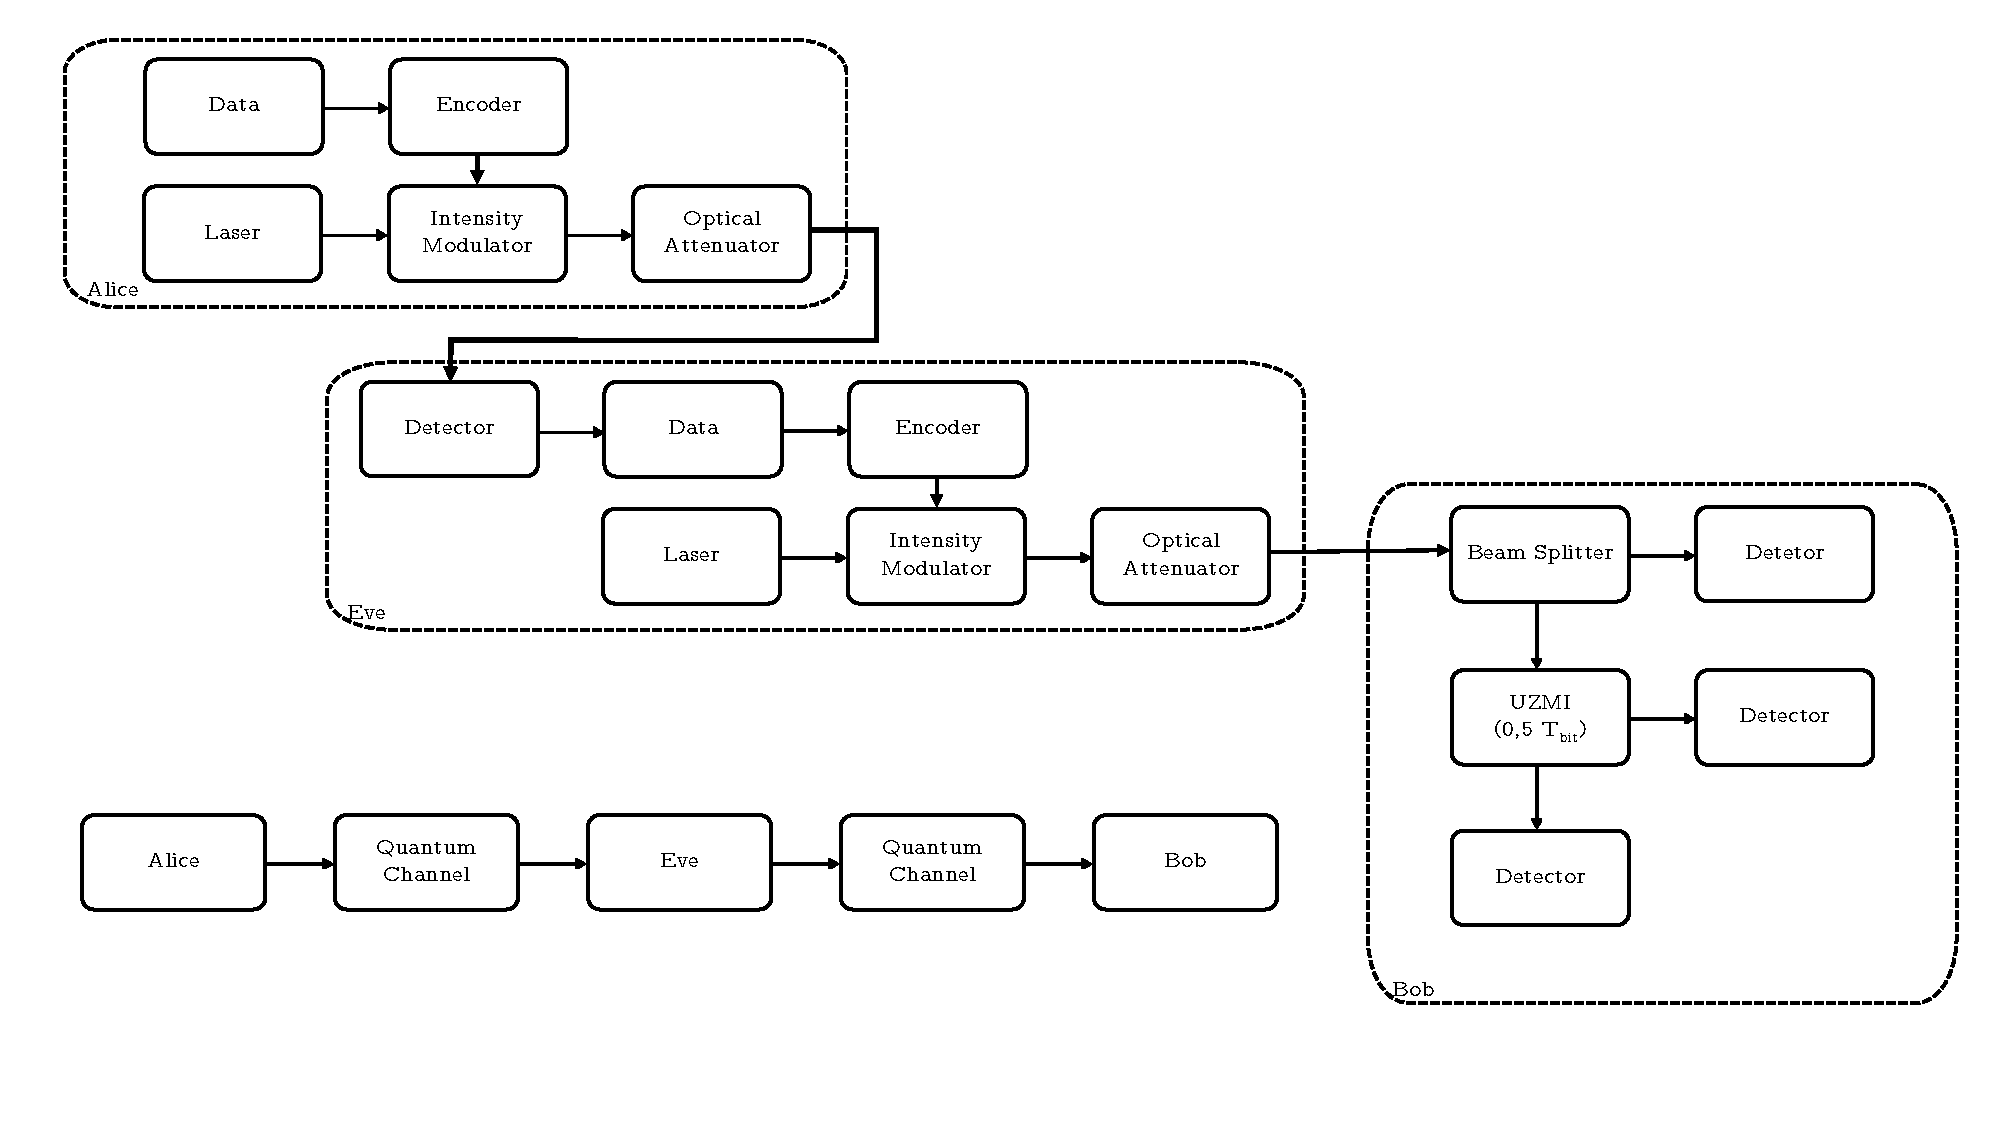
\includegraphics[width=0.55\textwidth]{./figures/Diagrama_de_blocos.pdf}

\end{multicols}    
%--------------------------------------------------------------------------------------------------
%------------ SLIDE -------------------------------------------------------------------------------
\mysection{\Huge\textbf{Simulation}} \Large \vspace*{1cm}

For the Simulation, using a fiber without looses:
\begin{table}[hbt!]
\centering
\Large
\begin{tabular}{|c|c|}
\hline
\cellcolor[HTML]{005288}\color{white} Logical Bits from Alice & $10^{7}$\\ \hline
\cellcolor[HTML]{005288}\color{white} Probability of Decoy & 10 \% \\ \hline
\cellcolor[HTML]{005288}\color{white} Alice Attenuation & 0.1\\ \hline
\cellcolor[HTML]{005288}\color{white} Bob Detectors Efficiency  & 10 \% \\ \hline
\cellcolor[HTML]{005288}\color{white} Bob DarkCount Probability & $10^{-5}$ \\ \hline
\cellcolor[HTML]{005288}\color{white} Average Over & 200 times\\ \hline
\cellcolor[HTML]{005288}\color{white} Percentage of the Key for QBER & 50 \% \\ \hline

\end{tabular}
\end{table}

Note that $10^7$ logical bits in a fiber with 90\% looses and with a attenuation from Alice equal to 0.1 is 1 second with the system working.

In a simulation without attack, and with this variables, the final information that Bob and Alice have is:

\begin{table}[hbt!]
\centering
\Large
\begin{tabular}{c|c|c|c|}
\cline{2-4}
\multicolumn{1}{l|}{} & \cellcolor[HTML]{005288}{\color[HTML]{FFFFFF} Min} & \cellcolor[HTML]{005288}{\color[HTML]{FFFFFF} Averag.} & \cellcolor[HTML]{005288}{\color[HTML]{FFFFFF} Max} \\ \hline
\multicolumn{1}{|c|}{\cellcolor[HTML]{005288}{\color[HTML]{FFFFFF} QBER}} & $9.9 \times 10^{-5}$ & 0.0001366 & 0.00018906 \\ \hline
\multicolumn{1}{|c|}{\cellcolor[HTML]{005288}{\color[HTML]{FFFFFF} $B_{M1}+B_{M2}$}} & 95294 & 96288 & 97069 \\ \hline
\multicolumn{1}{|c|}{\cellcolor[HTML]{005288}{\color[HTML]{FFFFFF} Key Length}} & 422730 & 423898 & 425281 \\ \hline
\end{tabular}
\end{table}
%--------------------------------------------------------------------------------------------------
%------------ SLIDE -------------------------------------------------------------------------------
\mysection{\Huge\textbf{IR - Eve Efficiency}} \Large \vspace*{1cm}
Using the Attenuation of Eve equal to 0.1, by changing the efficiency we get:

\begin{table}[hbt!]
\centering
\Large
\begin{tabular}{c|c|c|c|c|c|c|c|c|c|}
\cline{2-10}
 & \multicolumn{3}{c|}{\cellcolor[HTML]{005288}{\color[HTML]{FFFFFF} Eve Efficiency = 0.1}} & \multicolumn{3}{c|}{\cellcolor[HTML]{005288}{\color[HTML]{FFFFFF} Eve Efficiency = 0.5}} & \multicolumn{3}{c|}{\cellcolor[HTML]{005288}{\color[HTML]{FFFFFF} Eve Efficiency = 1}} \\ \cline{2-10} 
\multicolumn{1}{l|}{} & \cellcolor[HTML]{005288}{\color[HTML]{FFFFFF} Min} & \cellcolor[HTML]{005288}{\color[HTML]{FFFFFF} Averag.} & \cellcolor[HTML]{005288}{\color[HTML]{FFFFFF} Max} & \cellcolor[HTML]{005288}{\color[HTML]{FFFFFF} Min} & \cellcolor[HTML]{005288}{\color[HTML]{FFFFFF} Averag.} & \cellcolor[HTML]{005288}{\color[HTML]{FFFFFF} Max} & \cellcolor[HTML]{005288}{\color[HTML]{FFFFFF} Min} & \cellcolor[HTML]{005288}{\color[HTML]{FFFFFF} Averag.} & \cellcolor[HTML]{005288}{\color[HTML]{FFFFFF} Max} \\ \hline
\multicolumn{1}{|c|}{\cellcolor[HTML]{005288}{\color[HTML]{FFFFFF} QBER}} & 0.0020583 & 0.73014 & 1 & 0.0016881 & 0.22776 & 1 & 0.001729 & 0.0023946 & 0.00032631 \\ \hline
\multicolumn{1}{|c|}{\cellcolor[HTML]{005288}{\color[HTML]{FFFFFF} $B_{M1}+B_{M2}$}} & 0 & 1106 & 9261 & 0 & 4602 & 9383 & 8889 & 9173 & 9404 \\ \hline
\multicolumn{1}{|c|}{\cellcolor[HTML]{005288}{\color[HTML]{FFFFFF} Key Length}} & 85 & \cellcolor[HTML]{E5EAF4}4968 & 40642 & 91 &\cellcolor[HTML]{E5EAF4} 20361 & 40883 & 40034 &\cellcolor[HTML]{E5EAF4} 40438 & 40748 \\ \hline
\end{tabular}
\end{table}
\vspace*{0.5cm}
Simulation without attack again for comparison:
\begin{table}[hbt!]
\centering
\Large
\begin{tabular}{c|c|c|c|}
\cline{2-4}
\multicolumn{1}{l|}{} & \cellcolor[HTML]{005288}{\color[HTML]{FFFFFF} Min} & \cellcolor[HTML]{005288}{\color[HTML]{FFFFFF} Averag.} & \cellcolor[HTML]{005288}{\color[HTML]{FFFFFF} Max} \\ \hline
\multicolumn{1}{|c|}{\cellcolor[HTML]{005288}{\color[HTML]{FFFFFF} QBER}} & $9.9 \times 10^{-5}$ & 0.0001366 & 0.00018906 \\ \hline
\multicolumn{1}{|c|}{\cellcolor[HTML]{005288}{\color[HTML]{FFFFFF} $B_{M1}+B_{M2}$}} & 95294 & 96288 & 97069 \\ \hline
\multicolumn{1}{|c|}{\cellcolor[HTML]{005288}{\color[HTML]{FFFFFF} Key Length}} & 422730 &\cellcolor[HTML]{E5EAF4} 423898 & 425281 \\ \hline
\end{tabular}
\end{table}

\begin{description}
\centering
\item Eve presence lowers the Key length.
\end{description}

%--------------------------------------------------------------------------------------------------
%------------ SLIDE -------------------------------------------------------------------------------
\mysection{\Huge\textbf{IR - Eve Attenuation}} \Large \vspace*{1cm}
Assuming that Eve has 100 \% efficiency. By altering the value of her attenuation we get:

\begin{table}[hbt!]
\centering
\Large
\begin{tabular}{c|c|c|c|c|c|c|}
\cline{2-7}
 & \multicolumn{3}{c|}{\cellcolor[HTML]{005288}{\color[HTML]{FFFFFF} Eve Attenuation = 1.101}} & \multicolumn{3}{c|}{\cellcolor[HTML]{005288}{\color[HTML]{FFFFFF} Eve Attenuation = 2}} \\ \cline{2-7} 
\multicolumn{1}{l|}{} & \cellcolor[HTML]{005288}{\color[HTML]{FFFFFF} Min} & \cellcolor[HTML]{005288}{\color[HTML]{FFFFFF} Averag.} & \cellcolor[HTML]{005288}{\color[HTML]{FFFFFF} Max} & \cellcolor[HTML]{005288}{\color[HTML]{FFFFFF} Min} & \cellcolor[HTML]{005288}{\color[HTML]{FFFFFF} Averag.} & \cellcolor[HTML]{005288}{\color[HTML]{FFFFFF} Max} \\ \hline
\multicolumn{1}{|c|}{\cellcolor[HTML]{005288}{\color[HTML]{FFFFFF} QBER}} & 0.00011775 & 0.00017323 & 0.00022875 & $6.21\times 10^{-5}$ & $8.93\times 10^{-5}$ & 0.00011472 \\ \hline
\multicolumn{1}{|c|}{\cellcolor[HTML]{005288}{\color[HTML]{FFFFFF} $B_{M1}+B_{M2}$}} & 99146 &\cellcolor[HTML]{E5EAF4} 100632 & 101557 & 181047 &\cellcolor[HTML]{E5EAF4} 182217 & 183986 \\ \hline
\multicolumn{1}{|c|}{\cellcolor[HTML]{005288}{\color[HTML]{FFFFFF} Key Length}} & 423756 & 424850 & 426440 & 739744 & 741841 & 743701 \\ \hline
\end{tabular}
\end{table}
\vspace*{0.5cm}
Simulation without attack again for comparison:
\begin{table}[hbt!]
\centering
\Large
\begin{tabular}{c|c|c|c|}
\cline{2-4}
\multicolumn{1}{l|}{} & \cellcolor[HTML]{005288}{\color[HTML]{FFFFFF} Min} & \cellcolor[HTML]{005288}{\color[HTML]{FFFFFF} Averag.} & \cellcolor[HTML]{005288}{\color[HTML]{FFFFFF} Max} \\ \hline
\multicolumn{1}{|c|}{\cellcolor[HTML]{005288}{\color[HTML]{FFFFFF} QBER}} & $9.9 \times 10^{-5}$ & 0.0001366 & 0.00018906 \\ \hline
\multicolumn{1}{|c|}{\cellcolor[HTML]{005288}{\color[HTML]{FFFFFF} $B_{M1}+B_{M2}$}} & 95294 & \cellcolor[HTML]{E5EAF4}96288 & 97069 \\ \hline
\multicolumn{1}{|c|}{\cellcolor[HTML]{005288}{\color[HTML]{FFFFFF} Key Length}} & 422730 & 423898 & 425281 \\ \hline
\end{tabular}
\end{table}

\begin{description}
\centering
\item Eve presence increases the sum ($B_{M1}+B_{M2}$) when the Key Length is the correct, and lowers the Key Length when the Sum ($B_{M1}+B_{M2}$) is correct.
\end{description}
%-------------------------------------------------------------------
%------------ SLIDE ------------------------------------------------
\mysection{} \sffamily \Large
\vspace{-10mm}
\centerline{E-mail: joaoantonio@ua.pt}
\vspace*{7cm}
\begin{itemize}
	\item Ouellette, Jennifer. "Quantum key distribution." Industrial Physicist 10.6 (2004): 22-25.
	\item Gisin, Nicolas, et al. "Towards practical and fast quantum cryptography." arXiv preprint quant-ph/0411022 (2004).
	\item Branciard, Cyril, et al. "Zero-error attacks and detection statistics in the coherent one-way protocol for quantum cryptography." arXiv preprint quant-ph/0609090 (2006).
	\item Kronberg, Dmitry Anatol'evich, et al. "Analysis of coherent quantum cryptography protocol vulnerability to an active beam-splitting attack." Quantum Electronics 47.2 (2017): 163.
\end{itemize}

\end{document}
